\section{The main theorem}\label{sec:thm}

\begin{theorem}\label{thm:main}
If $b: \Z_{\geq 0}\to\Z$ satisfies 
\begin{enumerate}
    \item $b(0)$ is odd,
    \item $4\mid (\Delta b)(x)$ for all $x\in\mathbb{Z}_{\geq 0}$,
    \item $2^n\mid (\Delta^nb)(x)$ for all $n\geq 2$ and $x\in \mathbb{Z}_{\geq 0}$,
\end{enumerate}
then
$\xi_2(C_n^b)=\xi_2(C_n)=s_2(n+1)-1.$
\end{theorem}

To prove the main theorem, we modify the approach of Postnikov and Sagan with average weight functions $r_b(\mathcal{O}; x)$ attached to orbits of binary trees. Under their conditions, these functions were always odd-valued, whereas they are only integer-valued under the weaker conditions of Theorem \ref{thm:main}. We develop a method of analyzing their parity and show via induction that we have an odd number of minimal orbits with odd-valued average weight functions, which will prove the theorem.

\subsection{Binary trees and minimal orbits} \label{subsec:binarytrees}

In this section we reprove some important facts about binary trees.

\begin{definition}
A \emph{binary tree} is a rooted tree where each vertex has a left child, a right child, both children, or no children.
\end{definition}

Let $\mathcal{T}_n$ denote the set of binary trees on $n$ vertices. One of the interpretations of Catalan numbers is that $C_n=\lvert \mathcal{T}_n\rvert$. There is a symmetry group $G_n$ acting on $\mathcal{T}_n$, generated by reflections about a vertex which switch the left and right subtrees. An orbit of trees refers to an orbit under the action of $G_n$, which groups together binary trees which are isomorphic when the distinction between left and right is disregarded.

The following lemma was shown by Deutsch and Sagan \cite{deutsch2006congruences}.
\begin{lemma}
\label{lem:orbit sizes}
Let $\mathcal{O}$ be an orbit of the symmetry group $G_n$ on $\mathcal{T}_n$. Then $\lvert \mathcal{O}\rvert$ is of the form $2^t$ for a nonnegative integer $t$. Furthermore, $t\geq s=s_2(n+1)-1$, with equality for $(2s-1)!!$ orbits.
\end{lemma}

We will use \emph{minimal orbit} to refer to an orbit of the minimum possible size, which is $2^s$. The set of all orbits of $\mathcal{T}_n$ under $G_n$ is denoted $\mathcal{U}_n$, and the set of minimal orbits is denoted $\mathcal{U}^{\text{min}}_n$.

\begin{definition}
The \emph{complete binary tree of depth $k$} is the binary tree of $2^k-1$ vertices where each vertex in layer $0, 1, \dotsc, k-2$ has two children and each vertex in layer $k-1$ has no children.
\end{definition}
Note that complete binary trees are exactly the trees whose orbit consist of just one tree.

Now we have the following key result which describes the structure of minimal orbits of trees on $n$ vertices. (Recall that these are orbits of size $2^{s_2(n+1)-1}$.) This was done more generally for $q$-ary trees by Konvalinka \cite{konvalinka2007divisibility}.

\begin{theorem}[Structure of minimal orbits]
\label{thm:orbit structure}
Let $s=s(n+1)-1$ and $n+1=2^{k_1}+\dotsb+2^{k_{s+1}}$ be the binary expansion of $n+1$. Then all trees in an orbit of $\mathcal{U}_n^{\text{min}}$ may be constructed in the following manner: construct an arbitrary binary tree with $s$ vertices, and then attach completely symmetric trees of depth $k_1, \dotsc, k_{s+1}$ to the $s+1$ endpoints.
\end{theorem}

See Figure \ref{fig:minorbit} for an example. In constructing these minimal orbits, the $s$ vertices of the ``arbitrary binary tree'' will be marked black while the other vertices will be marked white.

\begin{figure}[h!]
\centering
    \begin{tikzpicture}[
    level distance=1cm,
    level 1/.style={sibling distance=4cm},
    level 2/.style={sibling distance=3cm},
    level 3/.style={sibling distance=1.5cm},
    level 4/.style={sibling distance=0.75cm},
    level 5/.style={sibling distance=0.375cm},
    level 6/.style={sibling distance=0.1875cm}]
      \node[black] {}
        child {node[black] {}
          child {node[white] {}
            child {node[white] {}
            child {node[white] {}
            child {node[white] {}
            child {node[white] {}}
            child {node[white] {}}}
            child {node[white] {}
            child {node[white] {}}
            child {node[white] {}}}
            }
            child {node[white] {}
            child {node[white] {}
            child {node[white] {}}
            child {node[white] {}}}
            child {node[white] {}
            child {node[white] {}}
            child {node[white] {}}}
            }
            }
            child {node[white] {}
            child {node[white] {}
            child {node[white] {}
            child {node[white] {}}
            child {node[white] {}}}
            child {node[white] {}
            child {node[white] {}}
            child {node[white] {}}}
            }
            child {node[white] {}
            child {node[white] {}
            child {node[white] {}}
            child {node[white] {}}}
            child {node[white] {}
            child {node[white] {}}
            child {node[white] {}}}
            }
            }
            }
          child {node[white] {}
          child {node[white] {}}
          child {node[white] {}}}
        }
        child {node[black] {}
        child {node[black, xshift=1.5cm] {}
        child {node[white] {}}
        child {node[white] {}
            child {node[white] {}
            child {node[white] {}
            child {node[white] {}}
            child {node[white] {}}}
            child {node[white] {}
            child {node[white] {}}
            child {node[white] {}}}
            }
            child {node[white] {}
            child {node[white] {}
            child {node[white] {}}
            child {node[white] {}}}
            child {node[white] {}
            child {node[white] {}}
            child {node[white] {}}}
            }
            }}
        };
    \end{tikzpicture}
\caption{An example for $n=54, n+1=2^5+2^4+2^2+2^1+2^0$.}
\label{fig:minorbit}
\end{figure}
Furthermore, this mapping can be reversed in the following way: for every vertex, color it white if the left and right subtrees at that vertex are isomorphic, and otherwise color it black. The black vertices are the original $s$ vertices and all white vertices are part of complete binary trees.

The symmetries of such trees are generated precisely by reflections about the original $s$ vertices (the ones marked in black).

\begin{remark}
In Theorem \ref{thm:orbit structure}, the term $2^0$ may appear in the binary expansion of $n+1$. This corresponds to an empty tree. In the example of Figure \ref{fig:minorbit}, all the black vertices have two children except for the third one from the left, which has only a right child. This is because the empty tree was assigned to its left child.
\end{remark}
\subsection{Mapping $\mathcal{F}$ to $2$-adic integers} \label{subsec:2-adics}

Let $\mathcal{F}$ denote the set of functions $f: \mathbb{Z}_{\geq 0}\to\mathbb{Z}$ such that $2^n\mid (\Delta^nf)(x)$ for all $n\geq 0$ and $x\in \mathbb{Z}_{\geq 0}$. Define the shift operator $S$ by
\[(Sf)(x)=f(x+1).\]

\begin{lemma}
\label{lem:productrule}
The product rule
\[\Delta^n(f\cdot g)=\sum_{k=0}^{n}\binom{n}{k}\Delta^{n-k}\left(S^k(f)\right)\Delta^k(g)\]
holds, which can be extended to multiple functions as
\[\Delta^n(f_1\dotsm f_m)=\sum_{a_1+\dotsb+a_m=n}\binom{n}{a_1, \dotsc, a_m}\Delta^{a_1}(S^{a_2+\dotsb+a_m}f_1)\cdot \Delta^{a_2}(S^{a_3+\dotsb+a_m}f_2)\dotsm \Delta^{a_m}(f_m).\]
\end{lemma}

\begin{lemma}
\label{lem:F closure}
The set $\mathcal{F}$ is closed under the following operations:
\[f\mapsto Sf, \quad (f, g)\mapsto f\cdot g, \quad \text{ and }\quad (f, g)\mapsto \langle f, g\rangle = \frac{f(x+1)g(x)+f(x)g(x+1)}{2}.\]
\end{lemma}
\begin{proof}
    Closure under $S$ is clear. For multiplication, we may use the product rule: each individual term in the expansion of $\Delta^n(f\cdot g)$ will be divisible by $2^n$. Likewise, by writing
    \[\langle f, g\rangle = f\cdot g + \frac{\Delta(f)\cdot g+f\cdot \Delta(g)}{2}\]
    and expanding with the product rule, we can show that $\langle f, g\rangle\in\mathcal{F}$ if $f, g\in\mathcal{F}$.
\end{proof}

Next, observe that for $f\in \mathcal{F}$ and any nonnegative integer $n$, we have $(\Delta^nf)(x)\equiv 0\pmod{2^n}$ by definition and also $(\Delta^{n+1}f)(x)\equiv 0\pmod{2^{n+1}}$. Then $\Delta^nf$ is constant modulo $2^{n+1}$ and must be equal to either $2^{n}$ or $0$. Define a mapping
\[\varepsilon: \mathcal{F}\to\{0, 1\}^{\mathbb{N}}\]
by sending $f$ to $(\varepsilon_0^f, \varepsilon_1^f, \dotsc)$ where 
\[
\varepsilon_n^f=\begin{cases}
0 & \text{ if }\Delta^nf\equiv 0\pmod {2^{n+1}} \\
1 & \text{ if }\Delta^nf\equiv 2^n\pmod{2^{n+1}}
\end{cases}.
\]

Define the weight of a binary tree $T$ by
\[w_b(T; x)=\prod_{v\in T}b(x+l_v)\]
where the product is over all vertices $v$ of $T$ and $l_v$ the number of left-edges in the path from the root to $v$. Evaluating this weight at $x=0$ and summing over all binary trees gives $C^b_n$. For each orbit $\mathcal{O}$, define a total weight function $w_{\mathcal{O}}(x)$ by
\[w_{\mathcal{O}}(x)=\sum_{T\in\mathcal{O}}w_b(T)\]
and the average weight function $r_b(\mathcal{O}; x)$ by
\[r_b(\mathcal{O}; x)=\frac{w_b(\mathcal{O}; x)}{\lvert\mathcal{O}\rvert}.\]
We have the recursive formula
\[r_b(\mathcal{O}; x)=b(x)\cdot\langle r_b(\mathcal{O}_L; x), r_b(\mathcal{O}_R; x)\rangle\]
(see Postnikov and Sagan \cite{postnikov2007power}) where $\mathcal{O}_L$ and $\mathcal{O}_R$ are the orbits associated to the left and right subtrees of the root. By Lemma \ref{lem:F closure} and induction, all functions $r_b(\mathcal{O}; x)$ are in $\mathcal{F}$.

\begin{definition}\label{def:epsilonO}
For an orbit $\mathcal{O}$ of binary trees, let $\varepsilon^{\mathcal{O}}_m=\varepsilon^f_m$ for $f=r_b(\O)\in \mathcal{F}$.
\end{definition}

From now on, we will also let $\varepsilon_k=\varepsilon^b_k$ for all $k$, i.e. the superscript $b$ will be omitted.

\begin{lemma}
\label{lem:epsilon formula}
For an orbit $\mathcal{O}$ with left and right orbits $\mathcal{O}_L, \mathcal{O}_R$, the following formula holds:
\[\varepsilon^{\mathcal{O}}_{m} \equiv\sum_{i+j+k=m}\binom{m}{i, j, k}\varepsilon_{k}(\varepsilon^{\mathcal{O}_L}_{i}\varepsilon^{\mathcal{O}_R}_j+\varepsilon^{\mathcal{O}_L}_{i+1}\varepsilon^{\mathcal{O}_R}_j+\varepsilon^{\mathcal{O}_L}_{i}\varepsilon^{\mathcal{O}_R}_{j+1})\pmod{2}.\]
\end{lemma}
\begin{proof}
    We make use of the identity 
    \[\langle f, g\rangle = f\cdot g + \frac{\Delta(f)\cdot g+f\cdot \Delta(g)}{2}.\]
    By expanding with the product rule, we have
    \begin{align*}
        \Delta^mr_b(\mathcal{O}; x)=\sum_{i+j+k=m} &\binom{m}{i, j, k}\Big[\Delta^k(S^{i+j}b)\cdot\Big(\Delta^{i}(S^jr_b(\mathcal{O}_L; x))\cdot \Delta^j(r_b(\mathcal{O}_R; x))+ \\
        &\frac{\Delta^{i+1}(S^jr_b(\mathcal{O}_L; x))\cdot \Delta^j(r_b(\mathcal{O}_R; x))+\Delta^{i}(S^jr_b(\mathcal{O}_L; x))\cdot \Delta^{j+1}(r_b(\mathcal{O}_R; x))}{2}\Big)\Big].
    \end{align*}
    We may now break this up into three sums, each of which will correspond to a term in the statement in the lemma. The first term is
    \[\sum_{i+j+k=m}\binom{m}{i, j, k}\Delta^k(S^{i+j}b)\cdot\Delta^{i}(S^jr_b(\mathcal{O}_L; x))\cdot \Delta^j(r_b(\mathcal{O}_R; x))\]
    As $b, r_b(\mathcal{O}_L; x), r_b(\mathcal{O}_R; x)\in \mathcal{F}$, each term in this summation is divisible by $2^k\cdot 2^i\cdot 2^j=2^m$. This term is \emph{not} divisible by $2^{m+1}$ if and only if all of the following hold:
    \begin{itemize}
        \item $\binom{m}{i, j, k}$ is odd.
        \item $\Delta^k(S^{i+j}b)\equiv 2^k\pmod{2^{k+1}}$.
        \item $\Delta^i(S^jr_b(\mathcal{O}_L; x))\equiv 2^i\pmod{2^{i+1}}$.
        \item $\Delta^{j}(r_b(\mathcal{O}_R; x))\equiv 2^j\pmod{2^{j+1}}$.
    \end{itemize}
    Therefore the residue modulo $2^{m+1}$ is equal to the residue of
    \[\sum_{i+j+k=m}\binom{m}{i, j, k}\varepsilon_k\varepsilon^{\mathcal{O}_L}_i\varepsilon^{\mathcal{O}_R}_{j}\]
    modulo $2$, multiplied by $2^m$.
    
    Similarly, the second term in the expansion is
    \[\frac{1}{2}\sum_{i+j+k=m}\binom{m}{i, j, k}\Delta^k(S^{i+j}b)\cdot\Delta^{i+1}(S^jr_b(\mathcal{O}_L; x))\cdot \Delta^j(r_b(\mathcal{O}_R; x)).\]
    The summation without the factor of $\frac{1}{2}$ is always a multiple of $2^{m+1}$, and will not be a multiple of $2^{m+2}$ if and only if $\binom{m}{i, j, k}$ is odd and $\varepsilon^b_k=\varepsilon^{\mathcal{O}_L}_{i+1}=\varepsilon^{\mathcal{O}_R}_{j}=1$. The third term can be handled similarly. Summing all the equations yields the lemma.
    
    In the case where $\mathcal{O}_L$ or $\mathcal{O}_R$ is empty, the associated function is $r_b=1$ with $\varepsilon^{r_b}_0=1$ and $\varepsilon^{r_b}_k=0$ for $k\geq 1$. The proof of the lemma works the same in this case.
\end{proof}

\begin{lemma}
    \label{lem:reduction}
    Let $\mathcal{O}$ be an orbit of binary trees on $n$ vertices, and suppose that for some vertex $v$, the subtree with root $v$ is a complete binary tree of depth $k$. Let $\mathcal{O}'$ be the same orbit of trees with the subtree at $v$ replaced by a single vertex at $v$. Then \[\varepsilon_m^{\mathcal{O}}=\varepsilon_0^{2^k-2}\varepsilon_m^{\mathcal{O}'}.\]
\end{lemma}

\begin{proof}
    We prove this lemma by induction. If $v$ is not the root vertex, then we use lemma \ref{lem:epsilon formula} to expand. Exactly one of the left and right subtrees contains $v$, so the inductive hypothesis applies to factor out $\varepsilon_0^{2^k-2}$. Hence we can reduce to the base case where $v$ is the root, i.e. we have a complete binary tree of depth $k$. To prove this case, we induct on $k$.
    
    For $k=1$ the lemma follows because $r_b(\mathcal{O}; x)=b(x)$. For the inductive step, we use Lemma \ref{lem:epsilon formula} where $\mathcal{O}_L$ and $\mathcal{O}_R$ are complete binary trees of depth $k-1$. Note that by symmetry of $i$ and $j$, the $\varepsilon^{\mathcal{O}_L}_{i+1}\varepsilon^{\mathcal{O}_R}_j+\varepsilon^{\mathcal{O}_L}_{i}\varepsilon^{\mathcal{O}_R}_{j+1}$ term cancels out in the sum, and $\varepsilon^{\mathcal{O}_L}_{i}\varepsilon^{\mathcal{O}_R}_j$ also cancels out for all terms where $i\neq j$. Finally, note that if $i=j > 0$, then the binomial coefficient $\binom{m}{i, j, k}=\binom{m}{k}\binom{i+j}{i}$ is divisible by $\binom{2i}{i}$, which is even. Therefore the only remaining term in the summation is the $i=j=0$ term. By the inductive hypothesis, we have
    \[\varepsilon^{\mathcal{O}}_m\equiv \varepsilon_m^{\mathcal{O'}}\varepsilon_0^{2(2^{k-1}-1)}=\varepsilon_0^{2^k-2}\varepsilon_m^{\mathcal{O}'}\]
    as desired.
\end{proof}

The recursive formula illustrated in Lemma~\ref{lem:epsilon formula} enables us to explicitly write down $\varepsilon_m^{\O}$ in an elegant way. This combinatorial description gives another quick proof to Lemma~\ref{lem:reduction} but is not used in other places of the paper. Readers are free to skip to the proof of the main theorem.

We view an orbit $\O$ as a rooted binary tree. Traditionally, we say that a vertex $v$ is a descendant of another vertex $w$ in $\O$ if the unique path connecting $v$ and the root passes through $w$. Similarly, we say that a vertex $v$ is a \textit{descendant} of an edge $e$ in $\O$ if the unique path connecting $v$ and the root contains $e$. In addition, we say that an edge $e$ of $\O$ connecting two vertices $u$ and $v$ \textit{originates from} $u$ if $v$ is a descendant of $e$ (or of $u$). Consequently, two edges $e$ and $e'$ are called \textit{siblings} if they originate from the same vertex.
\begin{definition}\label{def:coin}
A \textit{coin-configuration} $C$ on $\O$ of order $m$ consists of the following data:
\begin{itemize}
    \item a subset of edges $E$ of $\O$ such that no siblings are simultaneously selected,
    \item a distribution of distinct \textit{coins} $\{1,\ldots,m\}\cup E$ to all vertices of $\O$ such that each coin $c_e$ labeled by an edge $e\in E$ is assigned to a descendent of $e$.
\end{itemize}
For such a coin-configuration $C$, let $C_v$ denote the set of coins at $v$. Define its weight $\wt(C)=\prod_{v\in\O}\varepsilon_{|C_v|}$ where the product is over all vertices $v$ in $\O$. Moreover, let $\mathcal{C}^{\O}_m$ denote the set of all coin-configurations on $\O$ of order $m$. 
\end{definition}
See Figure~\ref{fig:coin} for an example of a coin-configuration of order 9 on an orbit $\O$ which is a rooted binary tree on 8 vertices, where the selected edges in $E$ are highlighted as thick line segments and the distribution of coins is written underneath the vertices. This particular example has weight $(\varepsilon_0)^2(\varepsilon_1)(\varepsilon_2)^4(\varepsilon_3)$.
\begin{figure}[h!]
\centering
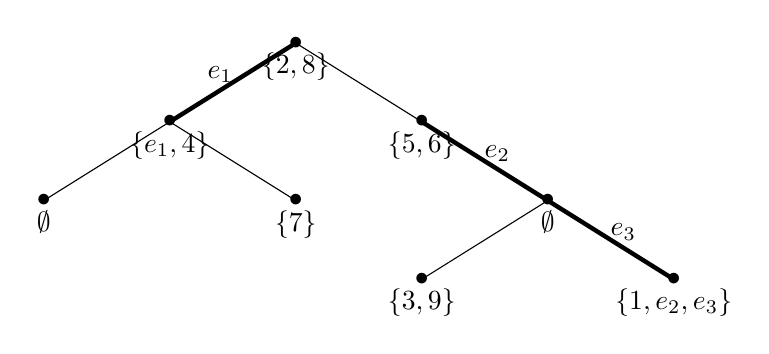
\begin{tikzpicture}[x=1.6cm]
\node at (0,0) {$\bullet$};
\node[below] at (0,0) {$\{2,8\}$};
\node at (-1,-1) {$\bullet$};
\node[below] at (-1,-1) {$\{e_1,4\}$};
\node at (-2,-2) {$\bullet$};
\node[below] at (-2,-2) {$\emptyset$};
\node at (0,-2) {$\bullet$};
\node[below] at (0,-2) {$\{7\}$};
\node at (1,-1) {$\bullet$};
\node[below] at (1,-1) {$\{5,6\}$};
\node at (2,-2) {$\bullet$};
\node[below] at (2,-2) {$\emptyset$};
\node at (3,-3) {$\bullet$};
\node[below] at (3,-3) {$\{1,e_2,e_3\}$};
\node at (1,-3) {$\bullet$};
\node[below] at (1,-3) {$\{3,9\}$};
\draw (-2,-2)--(-1,-1)--(0,0)--(1,-1)--(2,-2)--(3,-3);
\draw (0,-2)--(-1,-1);
\draw (2,-2)--(1,-3);
\draw[ultra thick] (0,0)--(-1,-1);
\draw[ultra thick] (1,-1)--(2,-2);
\draw[ultra thick] (2,-2)--(3,-3);
\node at (-0.6,-0.4) {$e_1$};
\node at (1.6,-1.4) {$e_2$};
\node at (2.6,-2.4) {$e_3$};
\end{tikzpicture}
\caption{An example of a coin-configuration of order 9 with weight $(\varepsilon_0)^2(\varepsilon_1)(\varepsilon_2)^4(\varepsilon_3)$.}
\label{fig:coin}
\end{figure}

\begin{proposition}\label{prop:coin}
We have the following explicit formula for an orbit $\O$:
$$\varepsilon_m^{\O}=\sum_{C\in\mathcal{C}^{\O}_m}\wt(C)$$
where the sum is over all coin-configurations $C$ on $\O$ of order $m$.
\end{proposition}
\begin{proof}
The proposition is a direct consequence of Lemma~\ref{lem:epsilon formula} and induction on the number of vertices of $\O$. For the base case where $\O$ is a single vertex, by definition, $\varepsilon^{\O}_m$ equals $\varepsilon_m$. At the same time, we have exactly 1 coin-configuration with weight $\varepsilon_m$ since there are no edges and all $m$ coins must be assigned to the unique vertex in $\O$.

Now assume that our proposition is true for all orbits with less than $n$ vertices and consider an orbit $\O$ with $n$ vertices. Similarly as in Lemma~\ref{lem:epsilon formula}, let $\O_L$ and $\O_R$ be the left and right subtrees of the root respectively and let $e_L$ and $e_R$ be the left and right edges originating from the root respectively. Consider $\sum_{C\in\mathcal{C}^{\O}_m}\wt(C)$, which is the RHS of the proposition. For a coin-configuration $C$ with a chosen subset $E$ of the edges, we cannot have both $e_L$ and $e_R$ lie in $E$. Then there are 3 possibilities: (1) $e_L\in E$, $e_R\notin E$; (2) $e_L\notin E$, $e_R\in E$; (3) $e_L,e_R\notin E$. For (1), we have $\binom{m}{i,j,k}$ ways to assign $k$ coins to the root, $i+1$ total coins to the left subtree ($i$ original coins in $\{1,\ldots,m\}$ and a new coin from $e_L$), and $j$ total coins to the right subtree. This provides a sum of $$\sum_{i+j+k=m}\binom{m} {i,j,k}\varepsilon_k\sum_{C\in\mathcal{C}^{\O_L}_{i+1}}\wt(C)\sum_{C\in\mathcal{C}^{\O_R}_{j}}\wt(C)=\sum_{i+j+k=m}\binom{m} {i,j,k}\varepsilon_k\varepsilon_{i+1}^{\O_L}\varepsilon_{j}^{\O_R}$$
by induction. Similarly handle case (2) and (3) and take the total sum $\sum_{C\in\mathcal{C}^{\O}_m}\wt(C)$, which is the exact same expression as RHS of Lemma~\ref{lem:epsilon formula} so it equals $\varepsilon_m^{\O}$ as desired.
\end{proof}

From the description of $\varepsilon_m^{\O}$ using coin-configurations (Definition~\ref{def:coin}), Lemma~\ref{lem:reduction} becomes immediate: if a vertex $v$ of $\O$ has isomorphic left and right subtrees, we can pair up coin-configurations with nontrivial coin assignments to descendents of $v$ by switching the left and right subtrees of $v$ and each pair of coin-configurations have the same weight.
\subsection{Proof of the Main Theorem}\label{subsec:proof}

Now we are ready to prove Theorem \ref{thm:main}.

\begin{proof}[Proof of Theorem \ref{thm:main}]
    We write
    \[C^b_n=\sum_{\mathcal{O}\in\mathcal{U}_n}\lvert \mathcal{O}\rvert\cdot r_b(\mathcal{O}; 0).\]
    From Lemma \ref{lem:orbit sizes}, $\lvert \mathcal{O}\rvert$ is always a power of two with exponent at least $s=s_2(n+1)-1$. We also know that $r_b(\mathcal{O}; 0)$ is always an integer and by definition, $r_b(\mathcal{O}; 0)$ is odd if and only if $\varepsilon^{\mathcal{O}}_0=1$. Then
    \[C^b_n\equiv \Big(\sum_{\mathcal{O}\in\mathcal{U}_n^{\text{min}}}\varepsilon^{\O}_0\Big)2^s\pmod{2^{s+1}},\]
    so it is equivalent to show that $\sum_{\mathcal{O}\in\mathcal{U}_n^{\text{min}}}\varepsilon^{\O}_0$ is odd.

    We use Theorem \ref{thm:orbit structure} to construct all minimal orbits of trees on $n$ vertices. By Corollary \ref{lem:reduction}, if we replace each complete binary tree of depth greater than $0$ by a single vertex, we get a new orbit of binary trees (on fewer vertices) which has the same sequence $\varepsilon^{\mathcal{O}}_m$, only reduced by a power of $\varepsilon_0$. This operation will be referred to as ``reduction.'' In Figure \ref{fig:oddcase}, have reduced the tree from Figure \ref{fig:minorbit} and obtained a new tree. Note that we have preserved the colors of the vertices, as we will need to refer to them later.
    
    \begin{figure}[h!]
    \centering
    \begin{tikzpicture}[
    level distance=1cm,
    level 1/.style={sibling distance=3cm},
    level 2/.style={sibling distance=2cm},
    level 3/.style={sibling distance=1.5cm},
    level 4/.style={sibling distance=0.75cm},
    level 5/.style={sibling distance=0.375cm},
    level 6/.style={sibling distance=0.1875cm}]
      \node[black] {}
        child {node[black] {}
          child {node[white] {}
            child {node[white] {}
            child {node[white] {}
            child {node[white] {}
            child {node[white] {}}
            child {node[white] {}}}
            child {node[white] {}
            child {node[white] {}}
            child {node[white] {}}}
            }
            child {node[white] {}
            child {node[white] {}
            child {node[white] {}}
            child {node[white] {}}}
            child {node[white] {}
            child {node[white] {}}
            child {node[white] {}}}
            }
            }
            child {node[white] {}
            child {node[white] {}
            child {node[white] {}
            child {node[white] {}}
            child {node[white] {}}}
            child {node[white] {}
            child {node[white] {}}
            child {node[white] {}}}
            }
            child {node[white] {}
            child {node[white] {}
            child {node[white] {}}
            child {node[white] {}}}
            child {node[white] {}
            child {node[white] {}}
            child {node[white] {}}}
            }
            }
            }
          child {node[white] {}
          child {node[white] {}}
          child {node[white] {}}}
        }
        child {node[black] {}
        child {node[black, xshift=1cm] {}
        child {node[white] {}}
        child {node[white] {}
            child {node[white] {}
            child {node[white] {}
            child {node[white] {}}
            child {node[white] {}}}
            child {node[white] {}
            child {node[white] {}}
            child {node[white] {}}}
            }
            child {node[white] {}
            child {node[white] {}
            child {node[white] {}}
            child {node[white] {}}}
            child {node[white] {}
            child {node[white] {}}
            child {node[white] {}}}
            }
            }}
        };
        
    \node[black, xshift=7cm] {}
        child {node[black] {}
          child {node[white] {}}
          child {node[white] {}
          }
        }
        child {node[black] {}
        child {node[black, xshift=1cm] {}
        child {node[white] {}}
        child {node[white] {}
            }
            }
        };
    \end{tikzpicture}
    \caption{The example tree from Figure \ref{fig:minorbit}, and its reduction on the right.}
    \label{fig:oddcase}
    \end{figure}
    
    We first consider the number of vertices remaining after reduction. If $n+1$ is odd, then there are $2s$ vertices remaining because there are $s$ nonempty complete binary trees being attached to $s$ vertices. If $n+1$ is even, then the number of remaining vertices is $2s+1$. In either case, let $k$ be the number of vertices of the trees of the minimal orbits after the reduction. With $\mathcal{U}_k$ as the set of orbits on $k$ vertices, let $f(\mathcal{O})$ denote the number of times an orbit $\mathcal{O}$ appears after reduction. Then we have
    \[\sum_{\mathcal{O}\in\mathcal{U}_n^{\text{min}}}\varepsilon^{\mathcal{O}}_0 = \varepsilon_0^{n-k}\sum_{\mathcal{O}\in \mathcal{U}_k}f(\mathcal{O})\varepsilon^{\mathcal{O}}_0.\]
    We want to determine the left hand side modulo $2$, so we can ignore all orbits for which $f(\mathcal{O})$ is even.
    
    In fact, we claim that those trees which remain (appear an odd number of times) are those representing minimal orbits of trees on $k$ vertices. Recall with Theorem \ref{thm:orbit structure} we assigned certain vertices as white and others as black, and we maintain this color scheme. After the reduction, we always have $s$ or $s+1$ white leaves attached to $s$ black vertices. See Table \ref{tab:reducedtrees} for an example, with all minimal orbits of trees on $14$ vertices shown with their reductions. In Table \ref{tab:reducedcount}, the counts of the resulting trees on $6$ vertices are recorded, and we can see that only three of them remain.
    
    \begin{table}[h]
    \centering
    \begin{tabular}{|c|c||c|c||c|c|} \hline
    Original tree & Reduction & Original Tree & Reduction & Original Tree & Reduction \\ \hline
    %1st
    \begin{tikzpicture}[
    level distance=1cm,
    level 1/.style={sibling distance=3cm},
    level 2/.style={sibling distance=1.5cm},
    level 3/.style={sibling distance=0.75cm},
    level 4/.style={sibling distance=0.375cm},
    scale = 0.5]
      \node[black] {}
        child {node[black] {}
          child {node[white, xshift=0.375cm] {}}
        }
        child {node[black] {}
        child {node[white] {}
        child {node[white] {}}
        child {node[white] {}}}
            child {node[white] {}
            child {node[white] {}
            child {node[white] {}}
            child {node[white] {}}}
            child {node[white] {}
            child {node[white] {}}
            child {node[white] {}}}}
        };
    \end{tikzpicture}
    &
    \begin{tikzpicture}[
    level distance=1cm,
    level 1/.style={sibling distance=3cm},
    level 2/.style={sibling distance=1.5cm},
    level 3/.style={sibling distance=0.75cm},
    level 4/.style={sibling distance=0.375cm},
    scale = 0.5]
        \node[xshift = 4cm, black] {}
        child {node[black] {}
          child {node[white, xshift=0.375cm] {}}
        }
        child {node[black] {}
        child {node[white] {}}
        child {node[white] {}}
        };
    \end{tikzpicture}
    
    &
    %7th
    \begin{tikzpicture}[
    level distance=1cm,
    level 1/.style={sibling distance=1.5cm},
    level 2/.style={sibling distance=1.5cm},
    level 3/.style={sibling distance=1.5cm},
    level 4/.style={sibling distance=0.75cm},
    level 5/.style={sibling distance=0.375cm},
    scale = 0.5]
      \node[black] {}
      child {node[white] {}}
        child {node[black] {}
        child {node[black, xshift=0.375cm] {}
        child {node[white] {}
        child {node[white] {}
        child {node[white] {}}
        child {node[white] {}}}
        child {node[white] {}
        child {node[white] {}}
        child {node[white] {}}}}
        child {node[white] {}
        child {node[white] {}}
        child {node[white] {}}}
        }
        };
    \end{tikzpicture}
    &
    \begin{tikzpicture}[
    level distance=1cm,
    level 1/.style={sibling distance=1.5cm},
    level 2/.style={sibling distance=1.5cm},
    level 3/.style={sibling distance=1.5cm},
    level 4/.style={sibling distance=0.75cm},
    level 5/.style={sibling distance=0.375cm},
    scale = 0.5]
        \node[black, xshift=4cm] {}
        child {node[white] {}}
        child {node[black] {}
        child {node[black, xshift = 0.375cm] {}
        child {node[white] {}}
        child {node[white] {}}
        }
        };
    \end{tikzpicture}
    
    &
    
    %13th
    \begin{tikzpicture}[
    level distance=1cm,
    level 1/.style={sibling distance=3.0cm},
    level 2/.style={sibling distance=1.5cm},
    level 3/.style={sibling distance=0.75cm},
    level 4/.style={sibling distance=0.375cm},
    level 5/.style={sibling distance=0.375cm},
    scale = 0.5]
      \node[black] {}
      child {node[white] {}
      child {node[white] {}}
      child {node[white] {}}
        }
        child {node[black] {}
        child {node[white] {}
        child {node[white] {}
        child {node[white] {}}
        child {node[white] {}}}
        child {node[white] {}
        child {node[white] {}}
        child {node[white] {}}}
        }
        child {node[black] {}
        child {node[white, xshift=-0.1875cm] {}}
        }
        };
    \end{tikzpicture}
    &
    \begin{tikzpicture}[
    level distance=1cm,
    level 1/.style={sibling distance=1.5cm},
    level 2/.style={sibling distance=1.5cm},
    level 3/.style={sibling distance=1.5cm},
    level 4/.style={sibling distance=0.75cm},
    level 5/.style={sibling distance=0.375cm},
    scale = 0.5]
        \node[black, xshift=4cm] {}
        child {node[white] {}}
        child {node[black] {}
        child {node[white] {}}
        child {node[black] {}
        child {node[white, xshift = -0.375cm] {}}
        }
        };
    \end{tikzpicture}
    \\ \hline
    
    %2nd
    \begin{tikzpicture}[
    level distance=1cm,
    level 1/.style={sibling distance=3cm},
    level 2/.style={sibling distance=1.5cm},
    level 3/.style={sibling distance=0.75cm},
    level 4/.style={sibling distance=0.375cm},
    scale = 0.5]
      \node[black] {}
        child {node[black] {}
          child {node[white, xshift=0.375cm] {}
          child {node[white] {}}
            child {node[white] {}}
            }
        }
        child {node[black] {}
        child {node[white] {}}
            child {node[white] {}
            child {node[white] {}
            child {node[white] {}}
            child {node[white] {}}}
            child {node[white] {}
            child {node[white] {}}
            child {node[white] {}}}}
        };
    \end{tikzpicture}
    &
    \begin{tikzpicture}[
    level distance=1cm,
    level 1/.style={sibling distance=3cm},
    level 2/.style={sibling distance=1.5cm},
    level 3/.style={sibling distance=0.75cm},
    level 4/.style={sibling distance=0.375cm},
    scale = 0.5]
        \node[xshift = 4cm, black] {}
        child {node[black] {}
          child {node[white, xshift=0.375cm] {}}
        }
        child {node[black] {}
        child {node[white] {}}
        child {node[white] {}}
        };
    \end{tikzpicture}
    
    &
    %8th
    \begin{tikzpicture}[
    level distance=1cm,
    level 1/.style={sibling distance=1.5cm},
    level 2/.style={sibling distance=1.5cm},
    level 3/.style={sibling distance=0.75cm},
    level 4/.style={sibling distance=0.75cm},
    level 5/.style={sibling distance=0.375cm},
    scale = 0.5]
      \node[black] {}
      child {node[white] {}
      child {node[white] {}
        child {node[white] {}}
        child {node[white] {}}}
        child {node[white] {}
        child {node[white] {}}
        child {node[white] {}}}
        }
        child {node[black] {}
        child {node[black, xshift=0.375cm] {}
        child {node[white] {}}
        child {node[white] {}
        child {node[white] {}}
        child {node[white] {}}}
        }
        };
    \end{tikzpicture}
    &
    \begin{tikzpicture}[
    level distance=1cm,
    level 1/.style={sibling distance=1.5cm},
    level 2/.style={sibling distance=1.5cm},
    level 3/.style={sibling distance=1.5cm},
    level 4/.style={sibling distance=0.75cm},
    level 5/.style={sibling distance=0.375cm},
    scale = 0.5]
        \node[black, xshift=4cm] {}
        child {node[white] {}}
        child {node[black] {}
        child {node[black, xshift = 0.375cm] {}
        child {node[white] {}}
        child {node[white] {}}
        }
        };
    \end{tikzpicture}
    
    &
    
    %14th
    \begin{tikzpicture}[
    level distance=1cm,
    level 1/.style={sibling distance=3.0cm},
    level 2/.style={sibling distance=1.5cm},
    level 3/.style={sibling distance=0.75cm},
    level 4/.style={sibling distance=0.375cm},
    level 5/.style={sibling distance=0.375cm},
    scale = 0.5]
      \node[black] {}
      child {node[white] {}
      child {node[white] {}
        child {node[white] {}}
        child {node[white] {}}}
        child {node[white] {}
        child {node[white] {}}
        child {node[white] {}}}
        }
        child {node[black] {}
        child {node[white] {}
        child {node[white] {}}
        child {node[white] {}}
        }
        child {node[black] {}
        child {node[white, xshift=-0.1875cm] {}}
        }
        };
    \end{tikzpicture}
    &
    \begin{tikzpicture}[
    level distance=1cm,
    level 1/.style={sibling distance=1.5cm},
    level 2/.style={sibling distance=1.5cm},
    level 3/.style={sibling distance=1.5cm},
    level 4/.style={sibling distance=0.75cm},
    level 5/.style={sibling distance=0.375cm},
    scale = 0.5]
        \node[black, xshift=4cm] {}
        child {node[white] {}}
        child {node[black] {}
        child {node[white] {}}
        child {node[black] {}
        child {node[white, xshift = -0.375cm] {}}
        }
        };
    \end{tikzpicture}
    \\ \hline
    
    %3rd
    \begin{tikzpicture}[
    level distance=1cm,
    level 1/.style={sibling distance=3cm},
    level 2/.style={sibling distance=1.5cm},
    level 3/.style={sibling distance=0.75cm},
    level 4/.style={sibling distance=0.375cm},
    scale = 0.5]
      \node[black] {}
        child {node[black] {}
          child {node[white, xshift=0.375cm] {}
          child {node[white] {}
            child {node[white] {}}
            child {node[white] {}}}
            child {node[white] {}
            child {node[white] {}}
            child {node[white] {}}}}
        }
        child {node[black] {}
        child {node[white] {}
        child {node[white] {}}
        child {node[white] {}}}
            child {node[white] {}}
        };
    \end{tikzpicture}
    &
    \begin{tikzpicture}[
    level distance=1cm,
    level 1/.style={sibling distance=3cm},
    level 2/.style={sibling distance=1.5cm},
    level 3/.style={sibling distance=0.75cm},
    level 4/.style={sibling distance=0.375cm},
    scale = 0.5]
        \node[xshift = 4cm, black] {}
        child {node[black] {}
          child {node[white, xshift=0.375cm] {}}
        }
        child {node[black] {}
        child {node[white] {}}
        child {node[white] {}}
        };
    \end{tikzpicture} 
    
    &
    %9th
    \begin{tikzpicture}[
    level distance=1cm,
    level 1/.style={sibling distance=1.5cm},
    level 2/.style={sibling distance=1.5cm},
    level 3/.style={sibling distance=1.5cm},
    level 4/.style={sibling distance=0.75cm},
    level 5/.style={sibling distance=0.375cm},
    scale = 0.5]
      \node[black] {}
      child {node[white] {}
      child {node[white] {}}
        child {node[white] {}}
        }
        child {node[black] {}
        child {node[black, xshift=0.375cm] {}
        child {node[white] {}
        child {node[white] {}
        child {node[white] {}}
        child {node[white] {}}}
        child {node[white] {}
        child {node[white] {}}
        child {node[white] {}}}}
        child {node[white] {}}
        }
        };
    \end{tikzpicture}
    &
    \begin{tikzpicture}[
    level distance=1cm,
    level 1/.style={sibling distance=1.5cm},
    level 2/.style={sibling distance=1.5cm},
    level 3/.style={sibling distance=1.5cm},
    level 4/.style={sibling distance=0.75cm},
    level 5/.style={sibling distance=0.375cm},
    scale = 0.5]
        \node[black, xshift=4cm] {}
        child {node[white] {}}
        child {node[black] {}
        child {node[black, xshift = 0.375cm] {}
        child {node[white] {}}
        child {node[white] {}}
        }
        };
    \end{tikzpicture}
    
    &
    
    %15th
    \begin{tikzpicture}[
    level distance=1cm,
    level 1/.style={sibling distance=3.0cm},
    level 2/.style={sibling distance=1.5cm},
    level 3/.style={sibling distance=0.75cm},
    level 4/.style={sibling distance=0.75cm},
    level 5/.style={sibling distance=0.75cm},
    scale = 0.5]
      \node[black] {}
      child {node[white] {}
      child {node[white] {}
        child {node[white] {}}
        child {node[white] {}}}
        child {node[white] {}
        child {node[white] {}}
        child {node[white] {}}}
        }
        child {node[black] {}
        child {node[white] {}
        }
        child {node[black] {}
        child {node[white, xshift=-0.1875cm] {}
        child {node[white] {}}
        child {node[white] {}}
        }
        }
        };
    \end{tikzpicture}
    &
    \begin{tikzpicture}[
    level distance=1cm,
    level 1/.style={sibling distance=1.5cm},
    level 2/.style={sibling distance=1.5cm},
    level 3/.style={sibling distance=1.5cm},
    level 4/.style={sibling distance=0.75cm},
    level 5/.style={sibling distance=0.375cm},
    scale = 0.5]
        \node[black, xshift=4cm] {}
        child {node[white] {}}
        child {node[black] {}
        child {node[white] {}}
        child {node[black] {}
        child {node[white, xshift = -0.375cm] {}}
        }
        };
    \end{tikzpicture}
    \\ \hline
    
    %4th
    \begin{tikzpicture}[
    level distance=1cm,
    level 1/.style={sibling distance=3cm},
    level 2/.style={sibling distance=3cm},
    level 3/.style={sibling distance=1.5cm},
    level 4/.style={sibling distance=0.75cm},
    level 5/.style={sibling distance=0.375cm},
    scale = 0.5]
      \node[black] {}
        child {node[black, xshift=0.75cm] {}
        child {node[white] {}}
        child {node[black] {}
        child {node[white] {}
        child {node[white] {}}
        child {node[white] {}}}
        child {node[white] {}
        child {node[white] {}
        child {node[white] {}}
        child {node[white] {}}}
        child {node[white] {}
        child {node[white] {}}
        child {node[white] {}}}}
        }
        };
    \end{tikzpicture}
    &
    \begin{tikzpicture}[
    level distance=1cm,
    level 1/.style={sibling distance=3cm},
    level 2/.style={sibling distance=3cm},
    level 3/.style={sibling distance=1.5cm},
    level 4/.style={sibling distance=0.75cm},
    level 5/.style={sibling distance=0.375cm},
    scale = 0.5]
        \node[black, xshift=4cm] {}
        child {node[black, xshift = 0.75cm] {}
        child {node[white] {}}
        child {node[black] {}
        child {node[white] {}}
        child {node[white] {}}
        }
        };
    \end{tikzpicture}
    
    &
    
    %10th
    \begin{tikzpicture}[
    level distance=1cm,
    level 1/.style={sibling distance=1.5cm},
    level 2/.style={sibling distance=1.5cm},
    level 3/.style={sibling distance=0.75cm},
    level 4/.style={sibling distance=0.75cm},
    level 5/.style={sibling distance=0.375cm},
    scale = 0.5]
      \node[black] {}
      child {node[white] {}
        }
        child {node[black] {}
        child {node[white] {}
        child {node[white] {}}
        child {node[white] {}}}
        child {node[black] {}
        child {node[white, xshift=-0.1875cm] {}
        child {node[white] {}
        child {node[white] {}}
        child {node[white] {}}}
        child {node[white] {}
        child {node[white] {}}
        child {node[white] {}}}}
        }
        };
    \end{tikzpicture}
    &
    \begin{tikzpicture}[
    level distance=1cm,
    level 1/.style={sibling distance=1.5cm},
    level 2/.style={sibling distance=1.5cm},
    level 3/.style={sibling distance=1.5cm},
    level 4/.style={sibling distance=0.75cm},
    level 5/.style={sibling distance=0.375cm},
    scale = 0.5]
        \node[black, xshift=4cm] {}
        child {node[white] {}}
        child {node[black] {}
        child {node[white] {}}
        child {node[black] {}
        child {node[white, xshift = -0.375cm] {}}
        }
        };
    \end{tikzpicture} & & \\ \hline
    
    %5th
    \begin{tikzpicture}[
    level distance=1cm,
    level 1/.style={sibling distance=3cm},
    level 2/.style={sibling distance=3cm},
    level 3/.style={sibling distance=1.5cm},
    level 4/.style={sibling distance=0.75cm},
    level 5/.style={sibling distance=0.375cm},
    scale = 0.5]
      \node[black] {}
        child {node[black, xshift=0.75cm] {}
        child {node[white] {}
        child {node[white] {}}
        child {node[white] {}}}
        child {node[black] {}
        child {node[white] {}}
        child {node[white] {}
        child {node[white] {}
        child {node[white] {}}
        child {node[white] {}}}
        child {node[white] {}
        child {node[white] {}}
        child {node[white] {}}}}
        }
        };
    \end{tikzpicture}
    &
    \begin{tikzpicture}[
    level distance=1cm,
    level 1/.style={sibling distance=3cm},
    level 2/.style={sibling distance=3cm},
    level 3/.style={sibling distance=1.5cm},
    level 4/.style={sibling distance=0.75cm},
    level 5/.style={sibling distance=0.375cm},
    scale = 0.5]
        \node[black, xshift=4cm] {}
        child {node[black, xshift = 0.75cm] {}
        child {node[white] {}}
        child {node[black] {}
        child {node[white] {}}
        child {node[white] {}}
        }
        };
    \end{tikzpicture}
    
    &
    
    %11th
    \begin{tikzpicture}[
    level distance=1cm,
    level 1/.style={sibling distance=1.5cm},
    level 2/.style={sibling distance=1.5cm},
    level 3/.style={sibling distance=0.75cm},
    level 4/.style={sibling distance=0.375cm},
    level 5/.style={sibling distance=0.375cm},
    scale = 0.5]
      \node[black] {}
      child {node[white] {}
        }
        child {node[black] {}
        child {node[white] {}
        child {node[white] {}
        child {node[white] {}}
        child {node[white] {}}}
        child {node[white] {}
        child {node[white] {}}
        child {node[white] {}}}
        }
        child {node[black] {}
        child {node[white, xshift=-0.1875cm] {}
        child {node[white] {}}
        child {node[white] {}}
        }
        }
        };
    \end{tikzpicture}
    &
    \begin{tikzpicture}[
    level distance=1cm,
    level 1/.style={sibling distance=1.5cm},
    level 2/.style={sibling distance=1.5cm},
    level 3/.style={sibling distance=1.5cm},
    level 4/.style={sibling distance=0.75cm},
    level 5/.style={sibling distance=0.375cm},
    scale = 0.5]
        \node[black, xshift=4cm] {}
        child {node[white] {}}
        child {node[black] {}
        child {node[white] {}}
        child {node[black] {}
        child {node[white, xshift = -0.375cm] {}}
        }
        };
    \end{tikzpicture} & & \\ \hline
    
    %6th
    \begin{tikzpicture}[
    level distance=1cm,
    level 1/.style={sibling distance=3cm},
    level 2/.style={sibling distance=3cm},
    level 3/.style={sibling distance=1.5cm},
    level 4/.style={sibling distance=0.75cm},
    level 5/.style={sibling distance=0.375cm},
    scale = 0.5]
      \node[black] {}
        child {node[black, xshift=0.75cm] {}
        child {node[white] {}
        child {node[white] {}
        child {node[white] {}}
        child {node[white] {}}}
        child {node[white] {}
        child {node[white] {}}
        child {node[white] {}}}}
        child {node[black] {}
        child {node[white] {}}
        child {node[white] {}
        child {node[white] {}}
        child {node[white] {}}}
        }
        };
    \end{tikzpicture}
    &
    \begin{tikzpicture}[
    level distance=1cm,
    level 1/.style={sibling distance=3cm},
    level 2/.style={sibling distance=3cm},
    level 3/.style={sibling distance=1.5cm},
    level 4/.style={sibling distance=0.75cm},
    level 5/.style={sibling distance=0.375cm},
    scale = 0.5]
        \node[black, xshift=4cm] {}
        child {node[black, xshift = 0.75cm] {}
        child {node[white] {}}
        child {node[black] {}
        child {node[white] {}}
        child {node[white] {}}
        }
        };
    \end{tikzpicture}
    
    &
    
    %12th
    \begin{tikzpicture}[
    level distance=1cm,
    level 1/.style={sibling distance=1.5cm},
    level 2/.style={sibling distance=0.75cm},
    level 3/.style={sibling distance=0.75cm},
    level 4/.style={sibling distance=0.75cm},
    level 5/.style={sibling distance=0.375cm},
    scale = 0.5]
      \node[black] {}
      child {node[white] {}
      child {node[white] {}}
      child {node[white] {}}
        }
        child {node[black] {}
        child {node[white] {}
        }
        child {node[black] {}
        child {node[white, xshift=-0.1875cm] {}
        child {node[white] {}
        child {node[white] {}}
        child {node[white] {}}}
        child {node[white] {}
        child {node[white] {}}
        child {node[white] {}}}}
        }
        };
    \end{tikzpicture}
    &
    \begin{tikzpicture}[
    level distance=1cm,
    level 1/.style={sibling distance=1.5cm},
    level 2/.style={sibling distance=1.5cm},
    level 3/.style={sibling distance=1.5cm},
    level 4/.style={sibling distance=0.75cm},
    level 5/.style={sibling distance=0.375cm},
    scale = 0.5]
        \node[black, xshift=4cm] {}
        child {node[white] {}}
        child {node[black] {}
        child {node[white] {}}
        child {node[black] {}
        child {node[white, xshift = -0.375cm] {}}
        }
        };
    \end{tikzpicture} & & \\ \hline
    \end{tabular}
    \caption{Reduction of minimal orbits of trees on $14$ vertices to orbits of trees on $6$ vertices.}
    \label{tab:reducedtrees}
\end{table}

\begin{table}[h]
    \centering
    \begin{tabular}{|c|c|}\hline
    Reduced Tree & Count (=$f(\O)$) \\ \hline
    \begin{tikzpicture}[
    level distance=1cm,
    level 1/.style={sibling distance=3cm},
    level 2/.style={sibling distance=1.5cm},
    level 3/.style={sibling distance=0.75cm},
    level 4/.style={sibling distance=0.375cm},
    scale = 0.5]
        \node[xshift = 4cm, black] {}
        child {node[black] {}
          child {node[white, xshift=0.375cm] {}}
        }
        child {node[black] {}
        child {node[white] {}}
        child {node[white] {}}
        };
    \end{tikzpicture} & $3=\dfrac{3!\cdot 4}{2^3}$ \\ \hline
    
    \begin{tikzpicture}[
    level distance=1cm,
    level 1/.style={sibling distance=3cm},
    level 2/.style={sibling distance=3cm},
    level 3/.style={sibling distance=1.5cm},
    level 4/.style={sibling distance=0.75cm},
    level 5/.style={sibling distance=0.375cm},
    scale = 0.5]
        \node[black, xshift=4cm] {}
        child {node[black, xshift = 0.75cm] {}
        child {node[white] {}}
        child {node[black] {}
        child {node[white] {}}
        child {node[white] {}}
        }
        };
    \end{tikzpicture} & $3=\dfrac{3!\cdot 4}{2^3}$ \\ \hline
    
    \begin{tikzpicture}[
    level distance=1cm,
    level 1/.style={sibling distance=1.5cm},
    level 2/.style={sibling distance=1.5cm},
    level 3/.style={sibling distance=1.5cm},
    level 4/.style={sibling distance=0.75cm},
    level 5/.style={sibling distance=0.375cm},
    scale = 0.5]
        \node[black, xshift=4cm] {}
        child {node[white] {}}
        child {node[black] {}
        child {node[black, xshift = 0.375cm] {}
        child {node[white] {}}
        child {node[white] {}}
        }
        };
    \end{tikzpicture} & $3=\dfrac{3!\cdot 4}{2^3}$ \\ \hline
    
    \begin{tikzpicture}[
    level distance=1cm,
    level 1/.style={sibling distance=1.5cm},
    level 2/.style={sibling distance=1.5cm},
    level 3/.style={sibling distance=1.5cm},
    level 4/.style={sibling distance=0.75cm},
    level 5/.style={sibling distance=0.375cm},
    scale = 0.5]
        \node[black, xshift=4cm] {}
        child {node[white] {}}
        child {node[black] {}
        child {node[white] {}}
        child {node[black] {}
        child {node[white, xshift = -0.375cm] {}}
        }
        };
    \end{tikzpicture} & $6=\dfrac{3!\cdot 8}{2^3}$ \\ \hline
    \end{tabular}
    \caption{Counts of the resulting reduced trees.}
    \label{tab:reducedcount}
\end{table}
    
    
    Let $M$ be the size of the orbit of a tree on $k$ vertices obtained by reduction. In the case where $k=2s$, we claim that the number of times a given orbit $\O$ appears is given by $\frac{s!M}{2^s}$. We can prove this by counting the number of trees on $n$ vertices to which this corresponds: we have $s!$ ways of placing complete binary trees on the $s$ white vertices and $M$ different ways to determine the underlying structure, which will count every corresponding tree on $n$ vertices $2^s$ times because each such tree has $2^s$ symmetries.
    
    Now we determine when this quantity is odd. We have
    \[\xi_2\left(\frac{s!M}{2^s}\right)=\xi_2(s!)+\xi_2(M)-\xi_2(2^s)=s-s_2(s)+\xi_2(M)-s=\xi_2(M)-s_2(s).\]
    This is odd if and only if $\xi_2(M)=s_2(s)$. Since $s_2(s)=s_2(2s+1)-1=s_2(k)-1$, this occurs if and only if we have a minimal orbit.
    
    Similarly, when $k=2s+1$, the number of times that a tree appears is given by $\frac{(s+1)!M}{2^s}$, which is odd only when we have a minimal orbit for the same reason.
    
    Up to now, we have shown that if $f(\mathcal{O})\geq 1$, i.e. an orbit of trees on $k$ vertices actually appears after the reduction operation, then $f(\mathcal{O})$ is even if $\mathcal{O}\not \in\mathcal{U}_k^{\text{min}}$. If $\mathcal{O}\in \mathcal{U}_k^{\text{min}}$, then $\mathcal{O}$ will be counted an odd number of times if we know how to assign the nodes as white/black to ``expand'' the tree back to the original size, though this still leaves out the possibility of multiple or no white/black assignments for $\O$. To finish the claim, we show that if $\mathcal{O}\in\mathcal{U}_k^{\text{min}}$, then there is a unique assignment of black and white nodes to $\O$ so that some orbits in $\mathcal{U}^{\text{min}}_n$ reduce to $\O$ with that color assignment. We know that nodes with no children after reduction must be white and those with at least one child must be black after reduction, which shows uniqueness. Using Theorem \ref{thm:orbit structure}, we may directly verify that trees in an orbit of $\mathcal{U}_k^{\text{min}}$ will always have a number of white nodes which is equal to or one more than the number of black nodes, so this coloring is always valid.
    
    With the claim, we now have
    \[\sum_{\mathcal{O}\in\mathcal{U}_n^{\text{min}}}\varepsilon^{\mathcal{O}}_0= \varepsilon_0^{n-k}\sum_{\mathcal{O}\in \mathcal{U}_k}f(\mathcal{O})\varepsilon^{\mathcal{O}}_0 \equiv\varepsilon^{n-k}_0\sum_{\mathcal{O}\in\mathcal{U}_k^{\text{min}}}\varepsilon^{\mathcal{O}}_0\pmod{2}\]
    so we may reduce to the case of $k$ vertices. We always have $k < n$ if $n\geq 2$ because $n+1\geq 3$, meaning that minimal orbits contain complete binary trees of depth greater than $1$ and the reduction operation always removes a positive number of vertices.
    
    For our base cases, we will eventually reduce to $n=1$ or $n=2$, where the statement is directly verified. Specifically, we have
    \begin{align*}
        \sum_{\mathcal{O}\in\mathcal{U}_1^{\text{min}}}\varepsilon^{\mathcal{O}}_0 &= \varepsilon_0, \\
        \sum_{\mathcal{O}\in\mathcal{U}_2^{\text{min}}}\varepsilon^{\mathcal{O}}_0 &= \varepsilon_0(\varepsilon_0+\varepsilon_1).
    \end{align*}
    The assumptions on $b$ are precisely that $\varepsilon_0=1$ and $\varepsilon_1=0$, so this is odd, as desired.
    
    Note that the reduction to a smaller case preserves parity, so we reduce to the $n=1$ or $n=2$ case according to the parity of $n$ at the start. Thus we actually get a stronger result: if we relax the condition $4\mid \Delta b$ to $2\mid \Delta b$, then $\xi_2(C^b_n)=\xi_2(C_n)$ holds for odd $n$, while $\xi_2(C^b_n) > \xi_2(C_n)$ for even $n$ if $4\nmid \Delta b$.
\end{proof}

An \cite{an2010combinatorial} previously determined necessary and sufficient conditions, conjectured by Konvalinka \cite{konvalinka2007divisibility}, under which a polynomial weight function $b(x)=b_0+b_1x+b_2x^2+\dotsb\in \mathbb{Z}[x]$ satisfies $\xi_2(C^b_n)=\xi_2(C_n)$. Inspired by his results, we make the following conjecture.
\begin{conjecture}
\label{conj:maingeneralization}
If $b: \Z_{\geq 0}\to\Z$ satisfies 
\begin{enumerate}
    \item $b(0)$ is odd,
    \item $2^{n-s_2(n)}\mid (\Delta^nb)(x)$ for all $n\geq 2$ and $x\in \mathbb{Z}_{\geq 0}$,
    \item $b(0)\equiv b(1)\pmod{4}$,
\end{enumerate}
then $\xi_2(C_n^b)=\xi_2(C_n)=s_2(n+1)-1.$
\end{conjecture}
We would be particularly interested in seeing a combinatorial proof of Conjecture \ref{conj:maingeneralization} as An's overall strategy was very computational in nature.